 \documentclass[12pt,letterpaper]{article}
\usepackage[utf8]{inputenc}
\usepackage[spanish, es-tabla]{babel}
\usepackage[version=3]{mhchem}
\usepackage[journal=jacs]{chemstyle}
\usepackage{amsmath}
\usepackage{amsfonts}
\usepackage{amssymb}
\usepackage{makeidx}
\usepackage{xcolor}
\usepackage{verbatim}
\usepackage[stable]{footmisc}
\usepackage[section]{placeins}
%Paquetes necesarios para tablas
\usepackage{longtable}
\usepackage{array}
\usepackage{xtab}
\usepackage{multirow}
\usepackage{colortab}
%Paquete para el manejo de las unidades
\usepackage{siunitx}
\sisetup{mode=text, output-decimal-marker = {,}, per-mode = symbol, qualifier-mode = phrase, qualifier-phrase = { de }, list-units = brackets, range-units = brackets, range-phrase = --}
\DeclareSIUnit[number-unit-product = \;] \atmosphere{atm}
\DeclareSIUnit[number-unit-product = \;] \pound{lb}
\DeclareSIUnit[number-unit-product = \;] \inch{"}
\DeclareSIUnit[number-unit-product = \;] \foot{ft}
\DeclareSIUnit[number-unit-product = \;] \yard{yd}
\DeclareSIUnit[number-unit-product = \;] \pint{pt}
\DeclareSIUnit[number-unit-product = \;] \quart{qt}
\DeclareSIUnit[number-unit-product = \;] \flounce{fl-oz}
\DeclareSIUnit[number-unit-product = \;] \ounce{oz}
\DeclareSIUnit[number-unit-product = \;] \degreeFahrenheit{\SIUnitSymbolDegree F}
\DeclareSIUnit[number-unit-product = \;] \degreeRankine{\SIUnitSymbolDegree R}
\DeclareSIUnit[number-unit-product = \;] \usgallon{galón}
\DeclareSIUnit[number-unit-product = \;] \uma{uma}
\DeclareSIUnit[number-unit-product = \;] \ppm{ppm}
\DeclareSIUnit[number-unit-product = \;] \eqg{eq-g}
\DeclareSIUnit[number-unit-product = \;] \normal{\eqg\per\liter\of{solución}}
\DeclareSIUnit[number-unit-product = \;] \molal{\mole\per\kilo\gram\of{solvente}}
\usepackage{cancel}
%Paquetes necesarios para imágenes, pies de página, etc.
\usepackage{graphicx}
\usepackage{lmodern}
\usepackage{fancyhdr}
\usepackage[left=4cm,right=2cm,top=3cm,bottom=3cm]{geometry}

%Instrucción para evitar la indentación
%\setlength\parindent{0pt}
%Paquete para incluir la bibliografía
%\usepackage[backend=bibtex,style=chem-acs,biblabel=dot]{biblatex}
%\addbibresource{references.bib}

%Formato del título de las secciones

\usepackage{titlesec}
\usepackage{enumitem}
\titleformat*{\section}{\bfseries\large}
\titleformat*{\subsection}{\bfseries\normalsize}

%Creación del ambiente anexos
\usepackage{float}
\floatstyle{plaintop}
\newfloat{anexo}{thp}{anx}
\floatname{anexo}{Anexo}
\restylefloat{anexo}
\restylefloat{figure}

%Modificación del formato de los captions
\usepackage[margin=10pt,labelfont=bf]{caption}

%Paquete para incluir comentarios
\usepackage{todonotes}

%Paquete para incluir hipervínculos
\usepackage[colorlinks=true, 
            linkcolor = blue,
            urlcolor  = blue,
            citecolor = black,
            anchorcolor = blue]{hyperref}


%%%%%%%%%%%%%%%%%%%%%%
%Inicio del documento%
%%%%%%%%%%%%%%%%%%%%%%

\begin{document}
\title{Control Automático\\Proyecto 2}

\author{German Monge Cerdas\\2015035612\\Adriana Rojas Mesén\\2014059900\\Jorge Rojas Meza\\201006018\\Julio Viveros Hernández\\200946192}
\date{\today}
\maketitle
\section{Introducción}
Se analizó en el laboratorio cierto sistema y se construyó su respuesta en frecuencia (Diagrama de Bode) en lazo abierto, la cual es la única información disponible para el diseño de los reguladores. Para el desarrollo de este segundo proyecto, es obligatorio utilizar Scilab. Además, se debe de generar un informe utilizando Latex en la plataforma \textit{Overleaf}.

\section{Problema}

Considere el Diagrama de Bode de la función de transferencia en lazo cerrado directo que se presenta en la \ref{fig:fig1}.\\

\begin{figure}[hbtp]
	\centering
	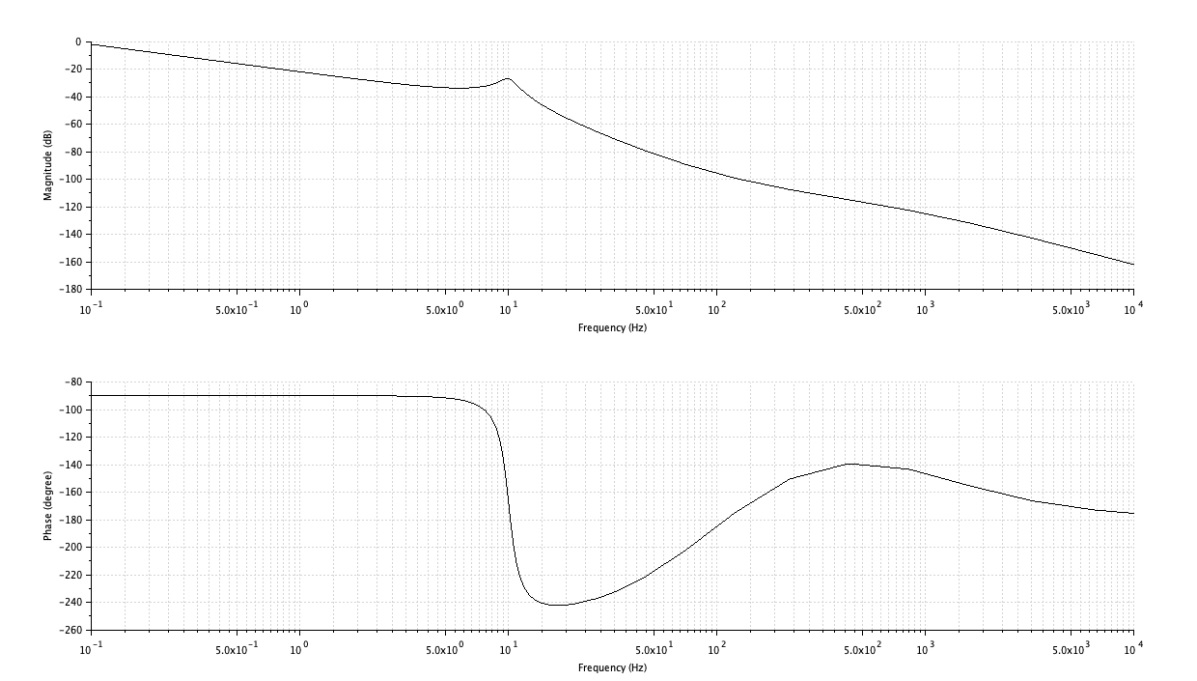
\includegraphics[width = \columnwidth]{Figura1.jpg} 
	\caption[Figura3]{Respuesta en frecuencia del sistema en análisis. [Fuente: enunciado del proyecto]} 
	\label{fig:fig1} 
\end{figure}

Se desean diseñar diferentes sistemas de control que se adapten y mejoren el comportamiento de lazo cerrado del mismo y que cumplan con las siguientes especificaciones:

\begin{itemize}
    \item Error cero cuando la referencia es un escalón.
    \item Error menor al 10$\%$ cuando la referencia es una rampa.
    \item Margen de fase mayor o igual a 60$^\circ$, de tal forma que al aproximar el sistema en lazo cerrado a un sistema de segundo orden se obtenga un sobreimpulso no mayor al 20$\%$.
\end{itemize}

El diagrama presentado en la \ref{fig:fig2} permite visualizar un acercamiento al pico máximo de resonancia del sistema y su respectiva frecuencia.\\

A continuación se presentan algunas relaciones de interés para el desarrollo de los diseños:\\

\begin{equation}
    \xi = \frac{MF}{100}
\end{equation}

\begin{equation}
    M_r = \frac{1}{2\xi\sqrt{1-\xi^2}}
\end{equation}

\begin{equation}
    \omega_r = \omega_n \sqrt{1-2\xi^2}
\end{equation}

\begin{equation}
    M_p = \exp^\frac{-\pi\xi}{\sqrt{1-\xi2}}
\end{equation}


\begin{equation}
    e_{ss}= \lim_{s \to 0} \frac{sR(s)}{1+G(s)H(s)}
\end{equation}


Donde $\xi$ es el factor de amortiguamiento, MF es el Margen de Fase, $M_r$ el pico máximo de ganancia a la frecuencia de resonancia $\omega_r$, $M_p$ el sobreimpulso y $e_{ss}$ el error de estado estacionario que depende de la entrada R(s). Se puede además, estimar de forma aproximada el tiempo de levantamiento como $t_r$ $\approx$ 1.8/$\omega_n$. Además, se recuerda que el ancho de banda se determina en la frecuencia de -3dB.\\

\begin{figure}[hbtp]
	\centering
	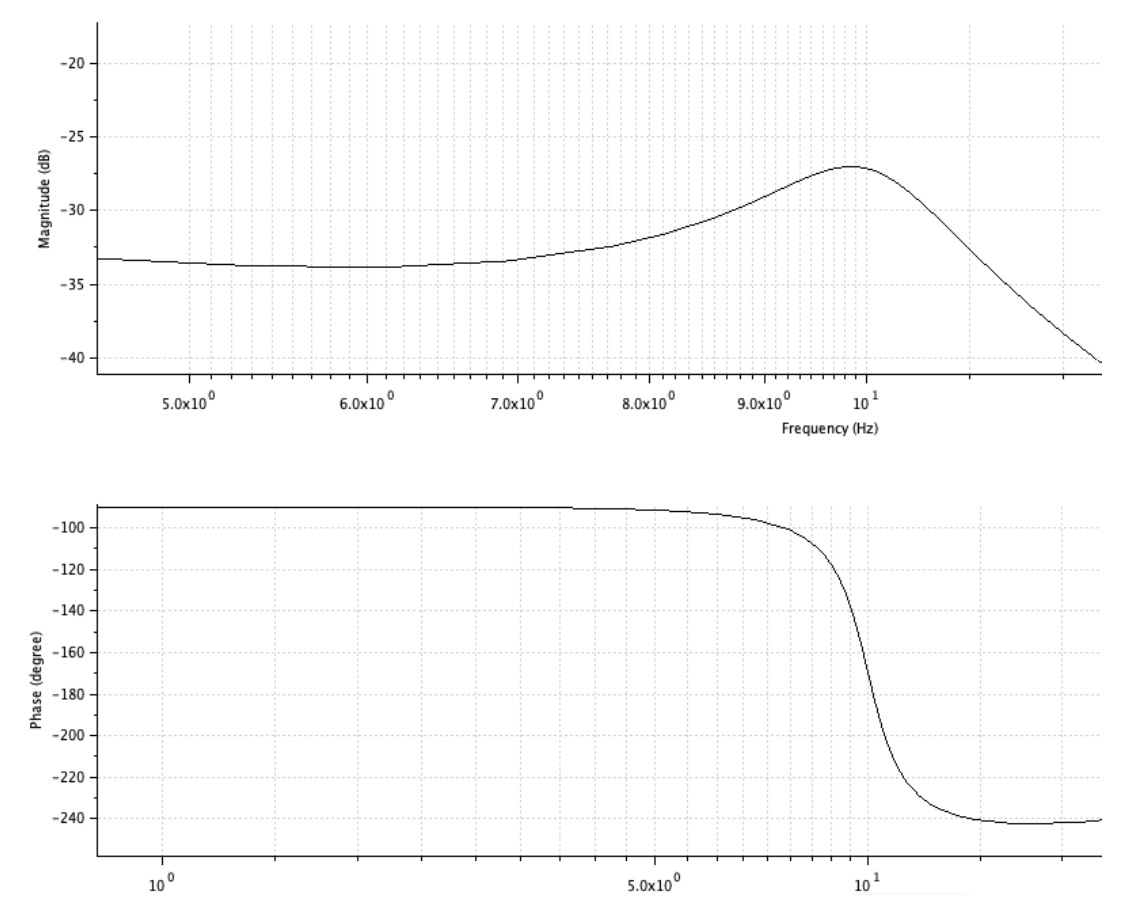
\includegraphics[width = \columnwidth]{Fig2.jpg} 
	\caption[Figura3]{Zoom del pico de resonancia máxima y su frecuencia. [Fuente: enunciado del proyecto]} 
	\label{fig:fig2} 
\end{figure}

\section{Cuestionamientos}

%------------------Inciso 1----------------%

\textbf{1.} Asumiendo que H(s) = 1. Encuentre la función de transferencia de lazo abierto a partir de los diagramas de Bode proporcionados.\\

\textbf{Solución}

\bigskip

Llámese a la función de transferencia buscada G(s). Tomando como base los puntos de interés marcados de la \ref{fig:fig1}, representados en la \ref{fig3}, y observándose que en el punto 1 (de la  \ref{fig3}), se puede observar que tenemos cuatro zonas de interés, las cuales son: 

\begin{itemize}
    \item un polo de orden dos, se encuentra debido al pico en el Bode de magnitud.
    \item se ubican dos ceros de orden uno porque en el Bode de fase se aprecia que a partir de cierto punto la fase sube considerablemente, esto no puede suceder con sólo un cero.
    \item un polo de orden uno, en el Bode de magnitud y fase se observa claramente el cambio de pendiente de las curvas a partir de cierto punto.
    \item un una ganancia que se le agrega al sistema, para que en una frecuencia de 0.01 Hz se obtenga alrededor de -2.5 dB.
\end{itemize}

\begin{figure}[hbtp]
	\centering
	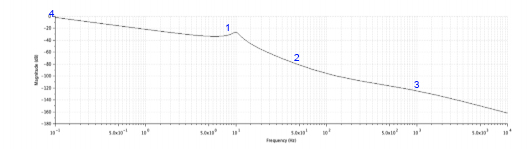
\includegraphics[width = \columnwidth]{diag3.jpg} 
	\caption[Figura3]{Respuesta en frecuencia del sistema en análisis con los puntos de interés [Fuente: propia]} 
	\label{fig3} 
\end{figure}

El polo de orden dos del punto 1) de la \ref{fig3} se obtiene utilizando las ecuaciones 2 y 3 con la \ref{fig:fig2}. Con la ecuación 6 se obtiene dicho polo, inicialmente se anota que la frecuencia $w_{r} = 9.833 Hz$, encontrada en la \ref{fig:fig2}, a partir de ahí se toman los siguientes datos.

\begin{equation*}
    M_r \approx -27,03125 dB
\end{equation*}

Sustituyendo el valor de $M_r$ en la ecuación (2) se tiene que:

\begin{equation*}
    \xi \approx -0.0839
\end{equation*}

De igual forma utilizando la ecuación (3), despejando $\omega_n$ con el valor de $\xi$ obtenido anteriormente:

\begin{equation*}
    \omega_n = 61.8059
\end{equation*}

\bigskip

Además obsérvese que el punto 1) es un polo doble, por lo tanto:

\begin{equation}
    G(s)= ((\frac{s}{\omega_n})^2 + 2\frac{\xi}{\omega_n}s +1) = ((\frac{s}{61.8059})^2 +2*\frac{-0.0839}{61.8059}s + 1)
\end{equation}


\bigskip

El punto 2) hace referencia a los ceros que levantan el Bode de fase, estos se encuentran trazando líneas rectas en la curva entre los puntos 1 y 3 con el fin de encontrar las zonas donde hay esquinas. Obtenemos dos puntos, los cuales son $7.777*10^1$ y $1.111*10^{2}$, estos serían los puntos con los cuales se construirán los ceros. Para ello, se utiliza la siguiente ecuación.

\begin{equation}
    cero = (1+\frac{s}{2*\pi*frecuencia[Hz]})
\end{equation}

\bigskip

Por lo tanto, tenemos los siguientes ceros: $(1+\frac{s}{2*\pi*7.777*10^1})$ y $(1+\frac{s}{2*\pi*1.111*10^{2}})$ .

\bigskip

Con el mismo método del punto 2) no se logró encontrar el polo escondido del punto 3), por lo que se decidió buscar un polo que logre satisfacer que en $10^4$ Hz la ganancia es de -175$^{\circ}$  y que el pico entre los ceros y el polo simple sea de una ganancia de aproximadamente -140$^{\circ}$.\\

La ganancia que genere una amplitud igual a la mostrada en el punto 4) se obtiene probando valores. Se observa que con un valor de $k = 0.45$ la curva de magnitud logra bajar hasta -2.5 dB aproximadamente.\\

La función de transferencia obtenida se muestra a continuación.

\begin{equation}
    G(s) = \frac{0.45\times(1+\frac{s}{2\pi\times7.77*10^1})\times(1+\frac{s}{2\pi\times1.111*10^2})}{s  \times  ((\frac{s}{61.8059})^2 + \frac{2*0.0839*s}{61.8059} +1) * (1+\frac{s}{2\pi*9*10^2})}
\end{equation}

\bigskip

Finalmente, la función de transferencia del sistema queda simplificada de la siguiente forma:

\begin{equation}
    G(s) = \frac{0.45+ 0.0009217s}{0.000000004629s^4+0.0002677s^3+0.0338937s^2 +s}
\end{equation}

\bigskip 

Para ingresar la Función de Transferencia a \textbf{Scilab} se utilizaron varios comandos. En primer lugar, para definir a la variable \textit{s} se usó:

\begin{verbatim}
    s= poly(0,'s')
\end{verbatim}

Una vez definido \textit{s} como variable de estado, se procedió a crear la función de transferencia como:

\begin{verbatim}
    Gs= syslin('c', G(s))
\end{verbatim}

Donde G(s) corresponde a la función de transferencia en la ecuación (7).\\

La función de transferencia de retroalimentación se obtiene usando el siguiente comando:

\begin{verbatim}
    FT_ret = FT/(1+FT)
\end{verbatim}

\bigskip

\bigskip

%------------------Inciso 2----------------%
\textbf{2.} Determine el error de estado estacionario del sistema.\\

\textbf{Solución}

\bigskip

\textbf{NOTA: G(s) = FT} para los archivos de Scilab.\\

Utilizando el comando para determinar el error de estado estacionario de \textbf{Scilab}, css:

\begin{verbatim}
    css = horner(s*FT*Rs, 0)
\end{verbatim}

\bigskip

Donde Rs es una entrada al sistema. Con un Rs de tipo escalón unitario $Rs = \frac{1}{s}$ y de tipo rampa $Rs = \frac{1}{s^2}$ se obtuvo que el error de estado estacionario es:
\begin{equation}
    e_{ss} \to \infty
\end{equation}

\bigskip

\bigskip

%------------------Inciso 3----------------%
\textbf{3.}  Determine el error en estado estacionario en lazo cerrado (Scilab).\\

\textbf{Solución}

\bigskip

Cerrando el lazo mediante:


\begin{verbatim}
    css = horner(s*Rs/(1+FT), 0)
\end{verbatim}

Para una entrada Rs de tipo escalón se tiene que el error en lazo cerrado es de:

\begin{equation}
    e_{ss} = 0
\end{equation}

\bigskip

De igual manera, para una entrada de tipo rampa se da un error en lazo cerrado de:

\begin{equation}
    e_{ss} = 2.222
\end{equation}

\bigskip

\bigskip

%------------------Inciso 4----------------%
\textbf{4.} Utilizando el Diagrama de Nyquist, evalúe la estabilidad en lazo cerrado $L(s) = G(s)H(s)$. (Scilab).\\

\textbf{Solución}

\bigskip

Para evaluar la estabilidad en lazo cerrado se ocupa saber si existe algún cero en el lado derecho del plano, para ello se obtiene el diagrama de Nyquist de la función en lazo abierto, así, de esta forma buscamos si el número de veces que se encierra el punto (-1, j0) es igual al número de polos que se encuentran en el semiplano derecho del plano S. Como se muestra en la imagen de la \ref{fig:fig4}, el punto (-1, j0) no esta encerrado y tampoco hay polos en el semiplano derecho, por lo tanto el sistema es estable. \\

El código utilizado para obtener el diagrama de Nyquist es el siguiente:  

\begin{verbatim}
    nyquist(FT_ret)    
\end{verbatim}

\begin{figure}[hbtp]
	\centering
	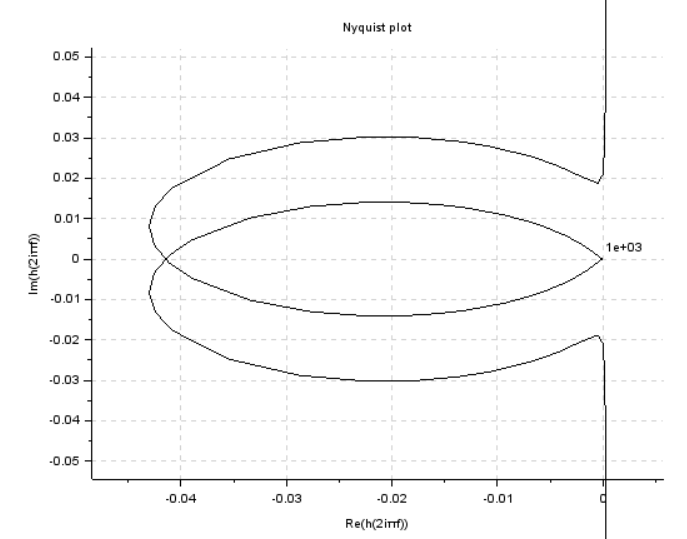
\includegraphics[width = .75 \columnwidth]{4nyquist_FT.png} 
	\caption[Figura3]{Diagrama de Nyquist para lazo abierto del sistema. [Fuente: propia, mediante Scilab]} 
	\label{fig:fig4} 
\end{figure}

\bigskip


%------------------Inciso 5----------------%
\textbf{5.} Diseñe un compensador tipo PD y evalúe la estabilidad del sistema para las entradas solicitadas, además corrobore si se cumplen las especificaciones de diseño a través de la carta de Nichols.\\

\textbf{Solución}

\bigskip

El compensador PD se construye de la siguiente manera: $PD = k*(s+z)$, donde $z = \frac{w_{c}}{tan \theta}$. El ángulo de fase máxima ($\theta$) se tomó como $90^{o}$ y $w_{c} = 1.012\times10^-1$. Observando que idealmente el Margen de Fase sea mayor a $60^{o}$, el sobreimpulso menor al 20$\%$ y el error generado por la rampa menor al 10\% se tiene que dicho compensador no era óptimo para proponerse, por lo tanto se generó un nuevo compensador PD al variar los datos de $K$ y $z$, el cual es mostrado a continuación:

\begin{equation}
    PD = 0.0004 * (s+2500)
\end{equation}

\bigskip

\textbf{Evaluación de estabilidad}

La estabilidad se evalúa con el diagrama de Nyquist y con cada entrada al sistema.

\bigskip

\textbf{Entrada escalón}

Se utilizan los siguientes comandos para obtener Nyquist:

\begin{verbatim}
    Rs = 1/s
    nyquist(PD*FT*1/s^1)
\end{verbatim}

\bigskip

La gráfica se muestra en la \ref{fig:fig5}. Como se puede observar, la traza no encierra el punto -1+j0, además, todos los polos de la función de transferencia L(s) están en el semiplano izquierdo del plano s.

\begin{figure}[hbtp]
	\centering
	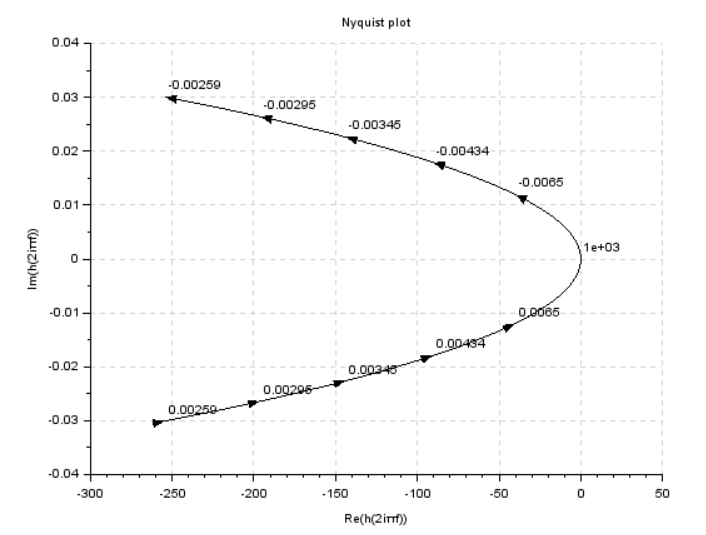
\includegraphics[width = 0.75 \columnwidth]{52escalon.png} 
	\caption[Figura3]{Diagrama de Nyquist para sistema con entrada escalón. [Fuente: propia, mediante Scilab]} 
	\label{fig:fig5} 
\end{figure}

\bigskip

\textbf{Entrada rampa}

Se utilizan los siguientes comandos para obtener Nyquist:

\begin{verbatim}
    Rs = 1/s^2  // Rampa
    nyquist(PD*FT*1/s^2)
\end{verbatim}

\bigskip

La gráfica se muestra en la \ref{fig:fig6}. Como se puede observar, la traza no encierra el punto -1+j0, similar al Nyquist de la entrada al escalón, el sistema es estable porque todos los polos de la función de transferencia L(s) se encuentran en el semiplano izquierdo del plano s.

\begin{figure}[hbtp]
	\centering
	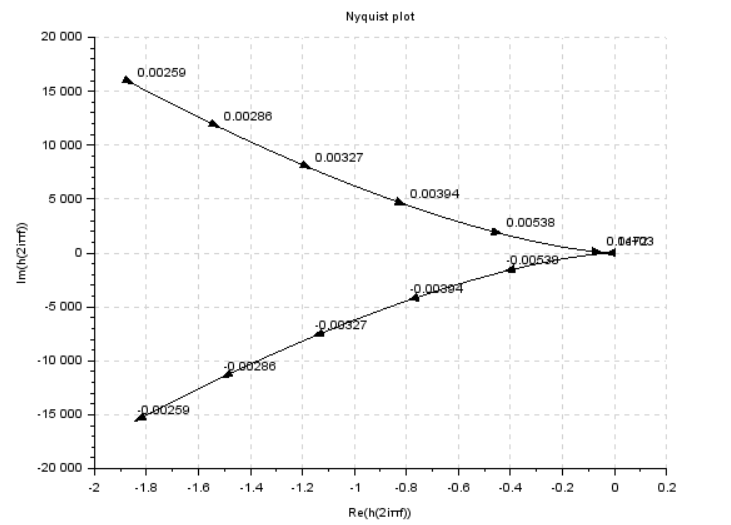
\includegraphics[width = 0.75 \columnwidth]{52rampa.png} 
	\caption[Figura3]{Diagrama de Nyquist para sistema con entrada rampa. [Fuente: propia, mediante Scilab]} 
	\label{fig:fig6} 
\end{figure}

\bigskip

\bigskip

\textbf{Carta de Nichols}

A partir del siguiente código se generó el diagrama de Nichols del sistema al agregar los controladores. Obsérvese la \ref{fig:fig7}.

\begin{verbatim}
    FT_PD = PD*FT
    black(FT_PD)
    nicholschart(colors=color('green')*[1,1])
\end{verbatim}

\begin{figure}[hbtp]
	\centering
	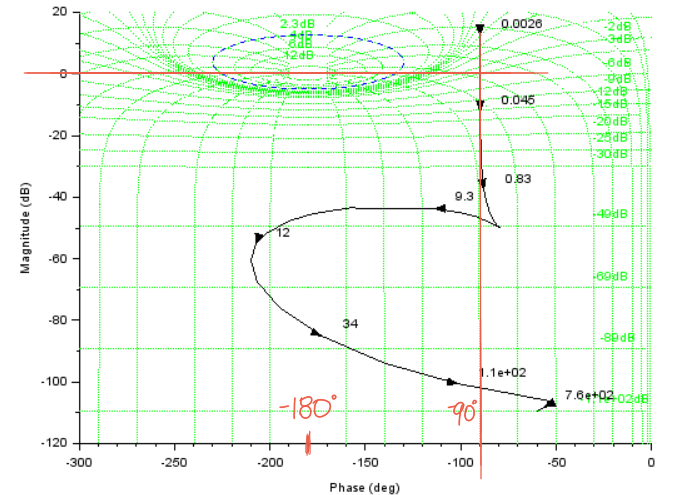
\includegraphics[width = 0.7 \columnwidth]{nichols2.png} 
	\caption[Figura7]{Carta de Nichols del sistema compensado. [Fuente: propia, mediante Scilab]} 
	\label{fig:fig7} 
\end{figure}

\bigskip

\bigskip

%------------------Inciso 6----------------%
\textbf{6.} Grafique la respuesta a las dos entradas solicitadas (escalón y rampa) con el compensador PD diseñado, además calcula el error de estado estacionario.\\

\textbf{Solución}

\bigskip

Los errores son obtenidos con los siguientes comandos.

\begin{verbatim}
    Rs = 1/s 
    c_ss = horner(s*Rs/(1+PD*FT),0)
    Rs = 1/s^2 // Rampa
    c_ss = horner(s*Rs/(1+PD*FT),0)
\end{verbatim}

Dando como resultado, para escalón $error = 0$ y para rampa $error = 2.222$.\\

Con entrada escalón se obtiene la respuesta mostrada en la \ref{fig:fig8}.\\

\begin{figure}[hbtp]
	\centering
	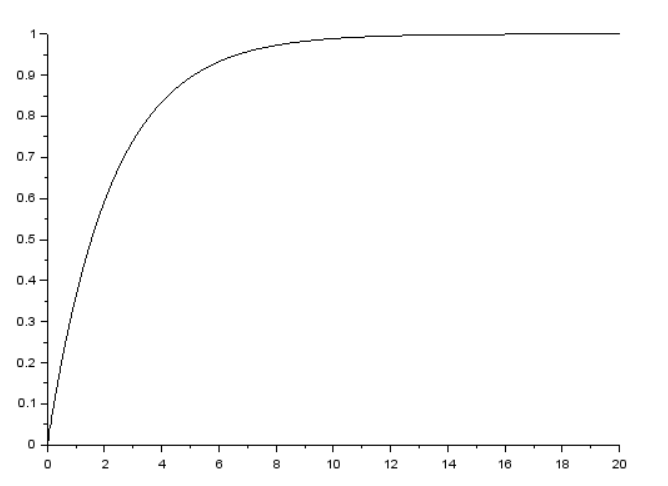
\includegraphics[width = .65 \columnwidth]{6escalon.png} 
	\caption[Figura7]{Respuesta con compensador PD con entrada escalón. [Fuente: propia]} 
	\label{fig:fig8} 
\end{figure}

Se observa que suavemente la curva tiende a 1, por lo tanto, el sistema con un compensador PD logra tener estabilidad con una entrada de tipo escalón.\\

Asimismo, con entrada rampa se obtiene la respuesta mostrada en la \ref{fig:fig9}.\\

\begin{figure}[hbtp]
	\centering
	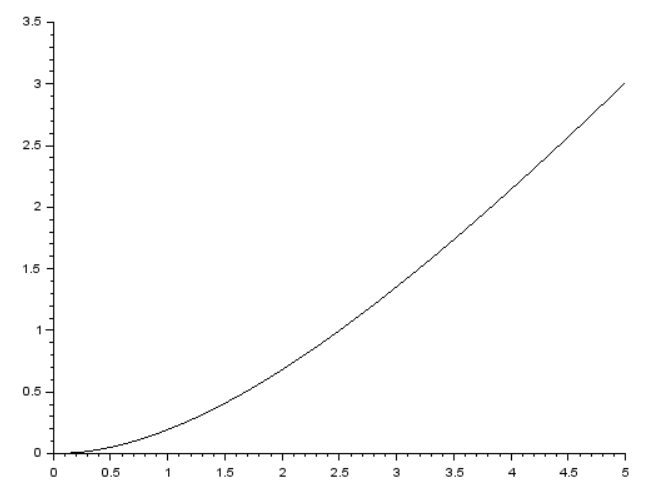
\includegraphics[width = .65 \columnwidth]{6rampa.png} 
	\caption[Figura7]{Respuesta con compensador PD con entrada rampa. [Fuente: propia]} 
	\label{fig:fig9} 
\end{figure}

Se aprecia que la curva tiene una ligera curva y no tiende a un número en específico, por lo tanto, el sistema con un compensador PD no logra tener estabilidad con una entrada de tipo rampa.

\bigskip

\bigskip

%------------------Inciso 7----------------%
\textbf{7.} Trace el diagrama de Bode de lazo cerrado con el compensador diseñado en (5) y compárelo con la carta de Nichols obtenida en (5) gráficamente. (Scilab).\\

\textbf{Solución}

\bigskip

En la \ref{fig:bodePD} se muestra el diagrama de Bode de lazo cerrado con el compensador tipo PD, en la \ref{fig:fig7} se muestra la carta de Nichols para el mismo compensador.

\begin{figure}[hbtp]
	\centering
	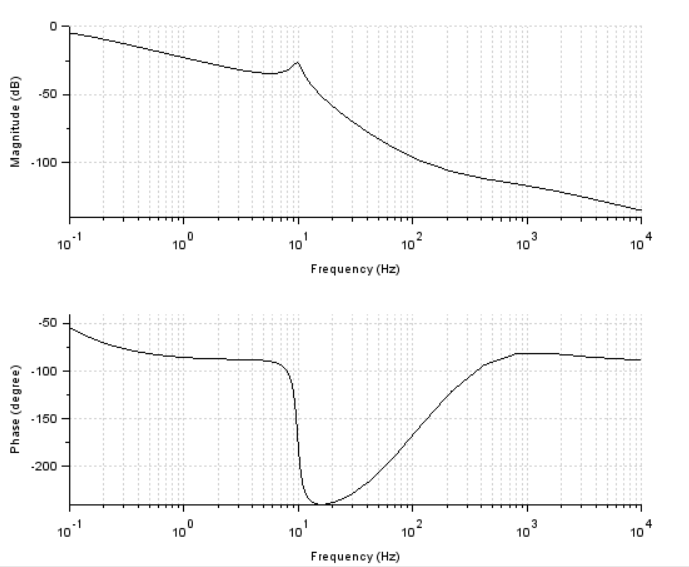
\includegraphics[width = .65 \columnwidth]{BodePD.png} 
	\caption[Figura7]{Bode del sistema en lazo cerrado con PD. [Fuente: propia]} 
	\label{fig:bodePD} 
\end{figure}

\bigskip

\bigskip

%------------------Inciso 8----------------%
\textbf{8.} Repita los puntos (5) y (6) para un compensador PI, PID, de adelanto y de atraso.\\

\textbf{Solución}

\bigskip

\textbf{1. Compensador PI}

\bigskip

Para el desarrollo del compensador PI se consideró que tiene que tener la forma $PI= PI = Kp * (s+Ki/Kp)/s$, donde se obtuvieron los factores Kp y Ki de manera que se cumplan los requisitos anteriormente mencionados. Se llegó a que el compensador corresponde a lo siguiente: $PI = 1 * (s+0.000005/1)/s$. 

\bigskip

\textbf{Evaluación de estabilidad}

\bigskip

Se utiliza el criterio de Nyquist para evaluar si la entrada es estable para el compensador PI con una entrada escalón. Esta respuesta se muestra en la \ref{fig:fig11}. De la misma manera se usa el criterio de Nyquist con una entrada rampa. La curva se muestra en la \ref{fig:fig12}.


\bigskip

\begin{figure}[hbtp]
	\centering
	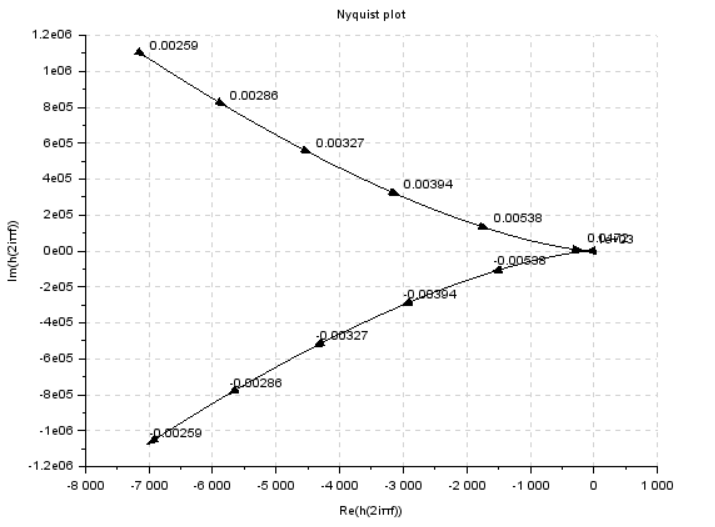
\includegraphics[width = .7 \columnwidth]{8a.png} 
	\caption[Figura7]{Nyquist para entrada escalón y un compensador PI. [Fuente: propia]} 
	\label{fig:fig11} 
\end{figure}


\begin{figure}[hbtp]
	\centering
	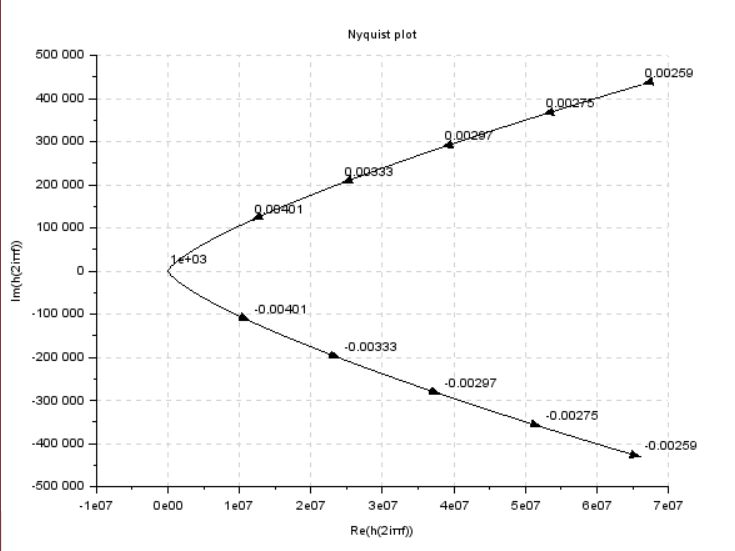
\includegraphics[width = .7 \columnwidth]{8b.png} 
	\caption[Figura7]{Nyquist para entrada rampa y un compensador PI. [Fuente: propia]} 
	\label{fig:fig12} 
\end{figure}

\bigskip

\textbf{Carta de Nichols}

Se generó la carta de Nichols del sistema con el compensador PI. Obsérvese la \ref{fig:NycholsPI}.

\begin{figure}[hbtp]
	\centering
	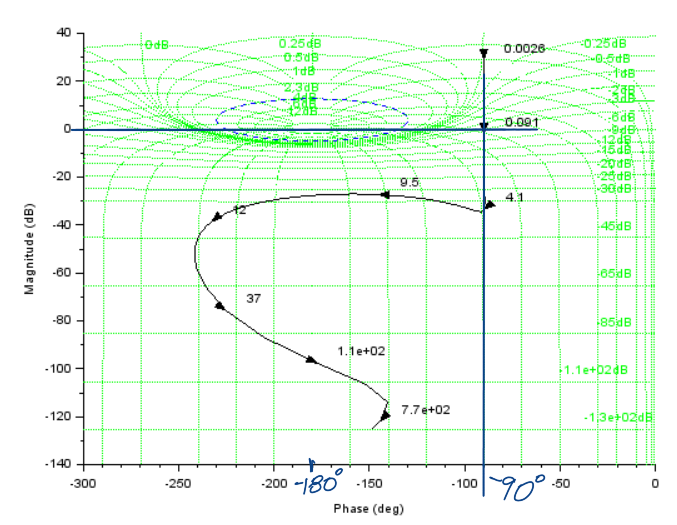
\includegraphics[width = 0.7 \columnwidth]{nicholsPI.png} 
	\caption[Figura7]{Carta de Nichols del sistema con PI. [Fuente: propia, mediante Scilab]} 
	\label{fig:NycholsPI} 
\end{figure}

\bigskip

Seguidamente se solicita graficar la respuesta a las dos entradas de referencia solicitadas (escalón y rampa) con el compensador PI diseñado. En la \ref{fig:PIesc} se muestra la respuesta del escalón y en la \ref{fig:PIram} la respuesta de la rampa.

\begin{figure}[hbtp]
	\centering
	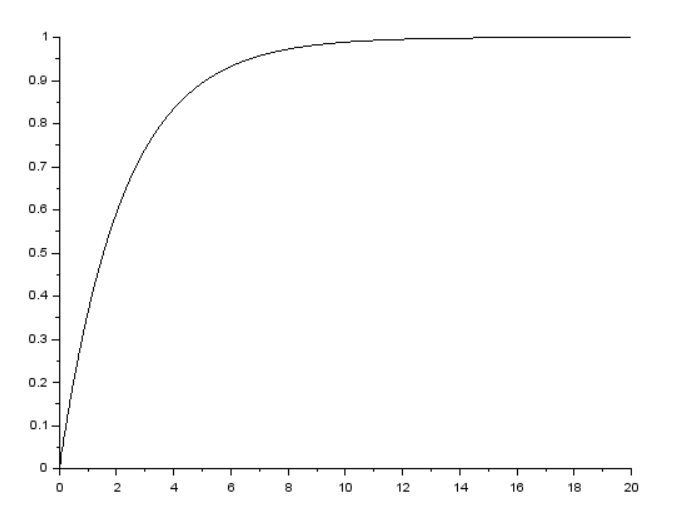
\includegraphics[width = 0.7 \columnwidth]{respuestaPIescalon.png} 
	\caption[Figura7]{Respuesta al escalón del sistema con PI [Fuente: propia, mediante Scilab]} 
	\label{fig:PIesc} 
\end{figure}

\begin{figure}[hbtp]
	\centering
	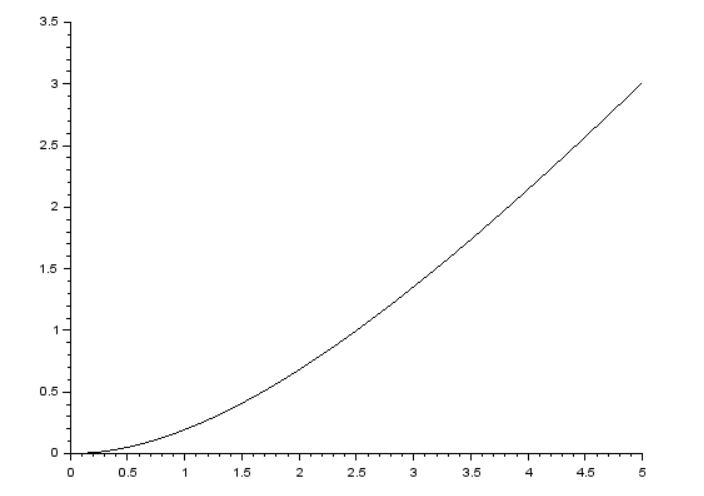
\includegraphics[width = 0.7 \columnwidth]{respuestaPIrampa.png} 
	\caption[Figura7]{Respuesta a la rampa del sistema con PI. [Fuente: propia, mediante Scilab]} 
	\label{fig:PIram} 
\end{figure}

Los errores de entrada escalón y rampa son obtenidos con los siguientes comandos.

\begin{verbatim}
    Rs = 1/s 
    c_ss = horner(s*Rs/(1+PI*FT),0)
    Rs = 1/s^2 // Rampa
    c_ss = horner(s*Rs/(1+PI*FT),0)
\end{verbatim}

Dando como resultado, para escalón $error = 0$ y para rampa $error = 0$.\\

\bigskip

Como último punto se solicita hacer una comparación del diagrama de Bode del sistema en lazo cerrado (\ref{fig:bodePI}) con la curva del diagrama de Nyquist encontrada en la \ref{fig:NycholsPI}.

\begin{figure}[hbtp]
	\centering
	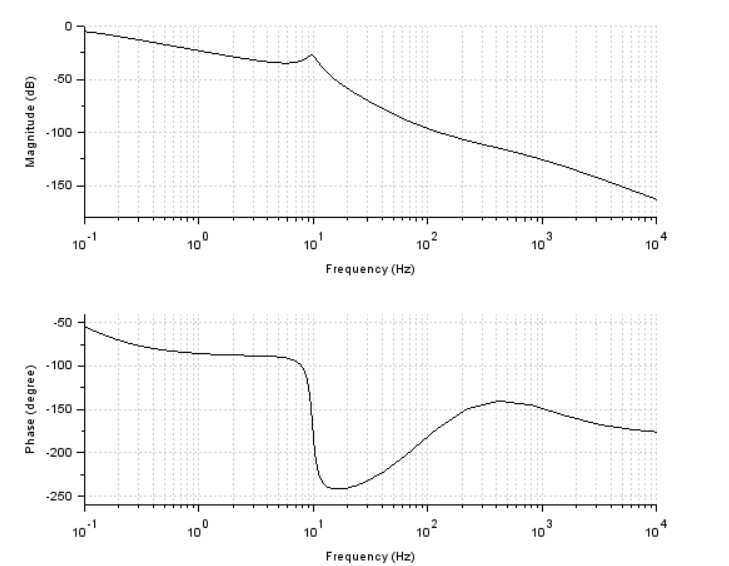
\includegraphics[width = 0.7 \columnwidth]{BodePI.png} 
	\caption[Figura7]{Diagrama de Bode del sistema con PI [Fuente: propia, mediante Scilab]} 
	\label{fig:bodePI} 
\end{figure}


\bigskip

\textbf{2. Compensador PID}

\bigskip

Para el compensador PID se utilizó la herramienta de Xcos de scilab, donde se logró llegar al sistema de la \ref{pidb} y este con los valores obtenidos de scilab para crear un PID, los cuales dieron kp=184.6, ki=1020, kd=4.717 y N= 7981, se usaron para llegar a la respuesta de la \ref{resppid}. \\

El error de estado estacionario para el PID en lazo cerrado tanto para entrada de rampa como entrada escalón fue de 0, el siguiente código fue el utilizado para obtener dicha respuesta:

\begin{verbatim}
    kp=184.6
    ki=1020
    kd=4.717
    n=7981
    PID=kp+(ki/s)+(kd*n/(1+7981/s))
    Rs = 1/s  // Escalón
    c_ss = horner(s*Rs/(1+FT*PID),0) // Luego de agregar retroalimentación
    disp(c_ss,"css escalon=")
    Rs = 1/s^2 // Rampa
    c_ss = horner(s*Rs/(1+FT*PID),0) // Luego de agregar retroalimentación
    disp(c_ss,"css rampa=")
\end{verbatim}

\begin{figure}[hbtp]
	\centering
	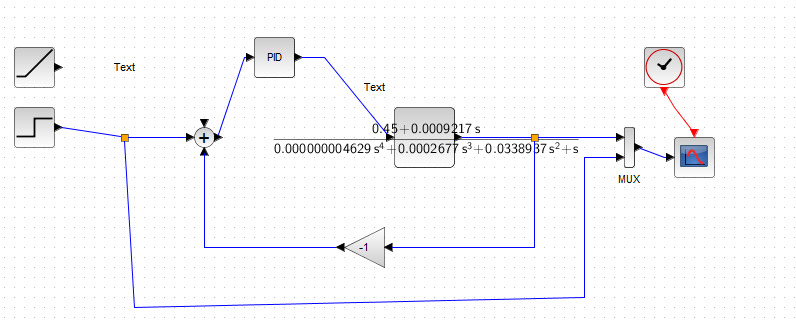
\includegraphics[width = .9 \columnwidth]{pidb.jpeg} 
	\caption[Figura7]{Diagrama del sistema para el compensador PID. [Fuente: propia, mediante Scilab]} 
	\label{pidb} 
\end{figure}

\begin{figure}[hbtp]
	\centering
	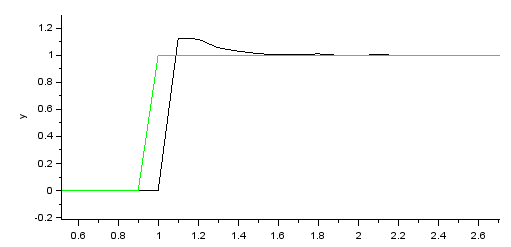
\includegraphics[width = .75 \columnwidth]{resppid.png} 
	\caption[Figura7]{Respuesta del compensador PID. [Fuente: propia, mediante Scilab]} 
	\label{resppid} 
\end{figure}

\begin{figure}[hbtp]
	\centering
	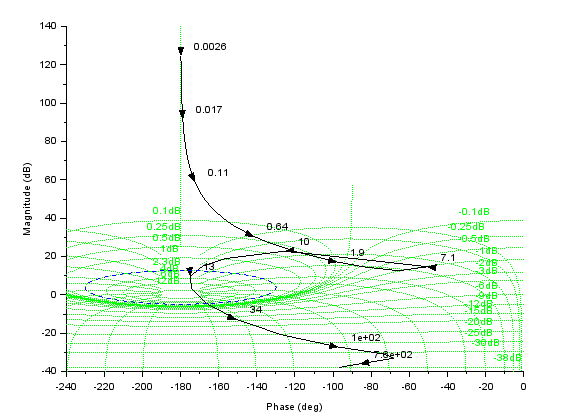
\includegraphics[width = .75 \columnwidth]{nicPID_.png} 
	\caption[Figura7]{Diagrama de Nichols para el PID. [Fuente: propia]} 
	\label{nicPID} 
\end{figure}

\begin{figure}[hbtp]
	\centering
	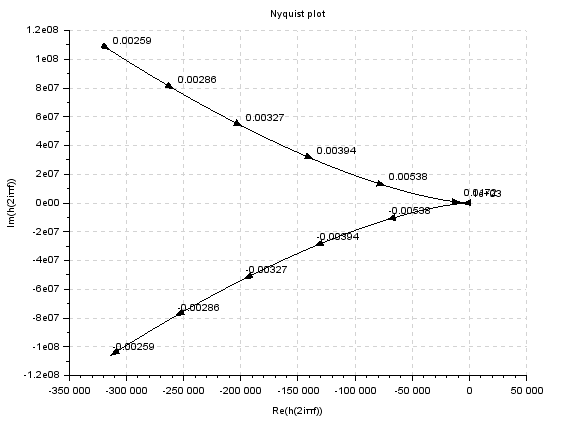
\includegraphics[width = 0.8 \columnwidth]{nyqpid.png} 
	\caption[Figura7]{Diagrama de Nyquist para el PID. [Fuente: propia]} 
	\label{nyqpid} 
\end{figure}

\begin{figure}[hbtp]
	\centering
	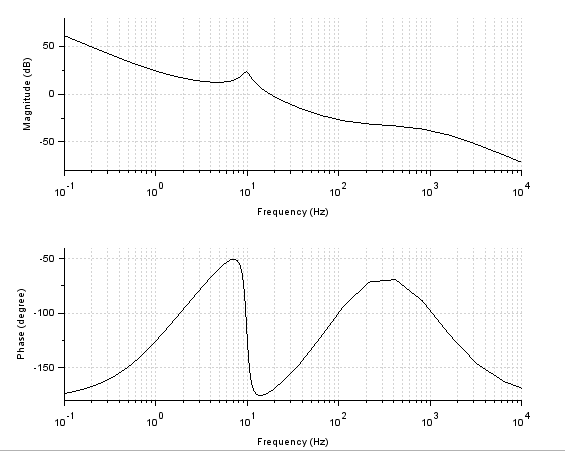
\includegraphics[width = .75 \columnwidth]{bodePID.png} 
	\caption[Figura7]{Diagrama de bode del PID. [Fuente: propia]} 
	\label{fig:fig10} 
\end{figure}

\bigskip

\bigskip


%----------------Inciso 9----------------%
\textbf{9.} Realice un análisis comparativo en el informe de los resultados obtenidos en los puntos del (5) al (7) entre los reguladores obtenidos.¿Cuál regulador es el mejor?\\

A continuación se adjunta una tabla resumen con los parámetros más importantes de los reguladores diseñados.


\begin{figure}[hbtp]
	\centering
	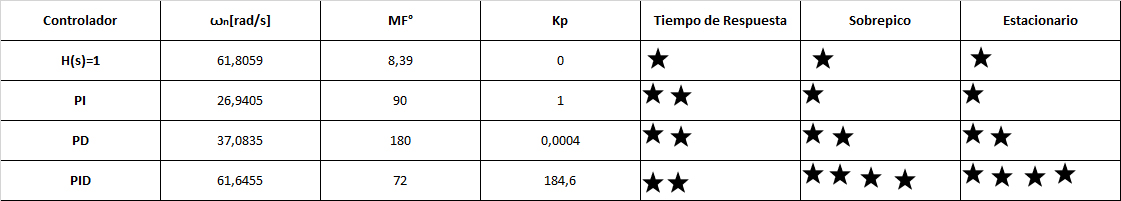
\includegraphics[width = .75 \columnwidth]{tabla.jpg} 
	\caption[Figura7]{Tabla Comparativa de los reguladores} 
	\label{fig:fig10} 
\end{figure}
 

\bigskip

\textbf{Solución}

\bigskip

\begin{thebibliography}{1}
\bibitem{Dorf}
Dorf, R and Bishop, R. \emph{Sistemas de Control Modernos}. Madrid: Pearson Educación. S.A., 10th ed., 2005.

\bibitem{Overleaf}
Extrído. \emph{Overleaf}. https://www.overleaf.com/. online, 2019.

\bibitem{Scilab}
Extrído. \emph{Scilab}. https://www.scilab.org/download/6.0.2. online, 2019.

\bibitem{Kuo} 
Kuo, B. \emph{Sistemas de Control Automático}. México: Prentice Hall, 7th ed., 1996.

\bibitem{Ogata} 
Ogata, K. (2010). \emph{Ingeniería de Control Moderna}. Madrid: Pearson Educación. S.A., 5th ed., 2010.

\end{thebibliography}


\nocite{*}
\bibliographystyle{ieeetr}
\bibliography{main.bib}
\end{document}
